\documentclass[aps,prl]{revtex4-2}
\usepackage{graphicx,amssymb,amsmath}
\bibliographystyle{apsrev4-2}
\renewcommand*{\citenumfont}[1]{S#1}
\renewcommand*{\bibnumfmt}[1]{[S#1]}


\begin{document}


\title{Supplementary Material\\Memory Matters for Cities}
\date{\today}
\author{Gezhi Xiu, Jianying Wang, Lei Dong}
% \email{xiugz@pku.edu.cn}
% \affiliation{IRSGIS, Peking University}

\author{Yu Liu}
\email{liuyu@urban.pku.edu.cn}
\affiliation{IRSGIS, Peking University, Beijing, China}
% \altaffiliation{CAMS (CNRS/EHESS) 190-198, avenue de France, 75244 Paris Cedex 13, France}

\pacs{} 

% If your reference list includes text notes as well as references,
% include the following line; otherwise, comment it out.


\maketitle
\tableofcontents
\vspace{1cm}

In this Supplementary Material, we provide details on ideas of model formulation, methodology, proofs, and empirical tests for the Letter Memory Matters for Cities.
\section{Details on the simulations}

The simulation results presented here are obtained in the following way. Instead of conducting the designed protocol, we do it in a equivalent way by stretching timeline to events labeled in integer. At each time step, we first decide if we add a new city, with probability $p(S)$, or a new meta-population to the existing city, with probability $1-p(S)$. The probability $p(S)$ is determined by the total 

The simulation results present in these supplementary materials are completed in the following way. We first obtain the (1) \emph{events} in the process and then label them with (2) timestamps. We first talk about how we label them. 

We denote the number of cities at the $n$th event as $k(n)$. We first determine the type of event, an establishment of a new city or an addition of meta-population. If it is an addition of 

\begin{figure}
	\centering
	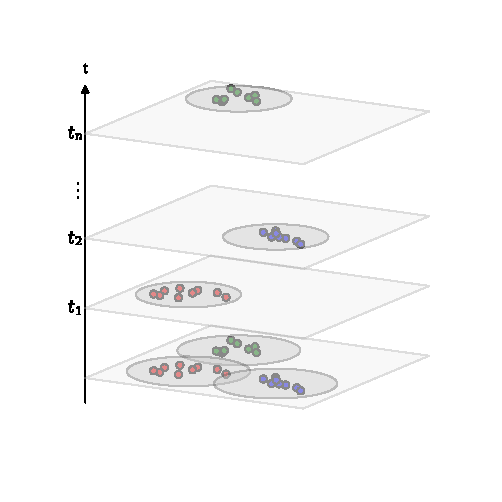
\includegraphics[width=0.5\linewidth]{./fig/mechan.pdf}
	\caption{The main idea of this model.}
\end{figure}

\section{Phase one: free growth phase}

Phase one of urban growth is in dealing with the case that urban growth over a given space. We focus on the more coming of urban population.

\subsection{Intrusion probability}

\begin{figure}[b]
	\centering
	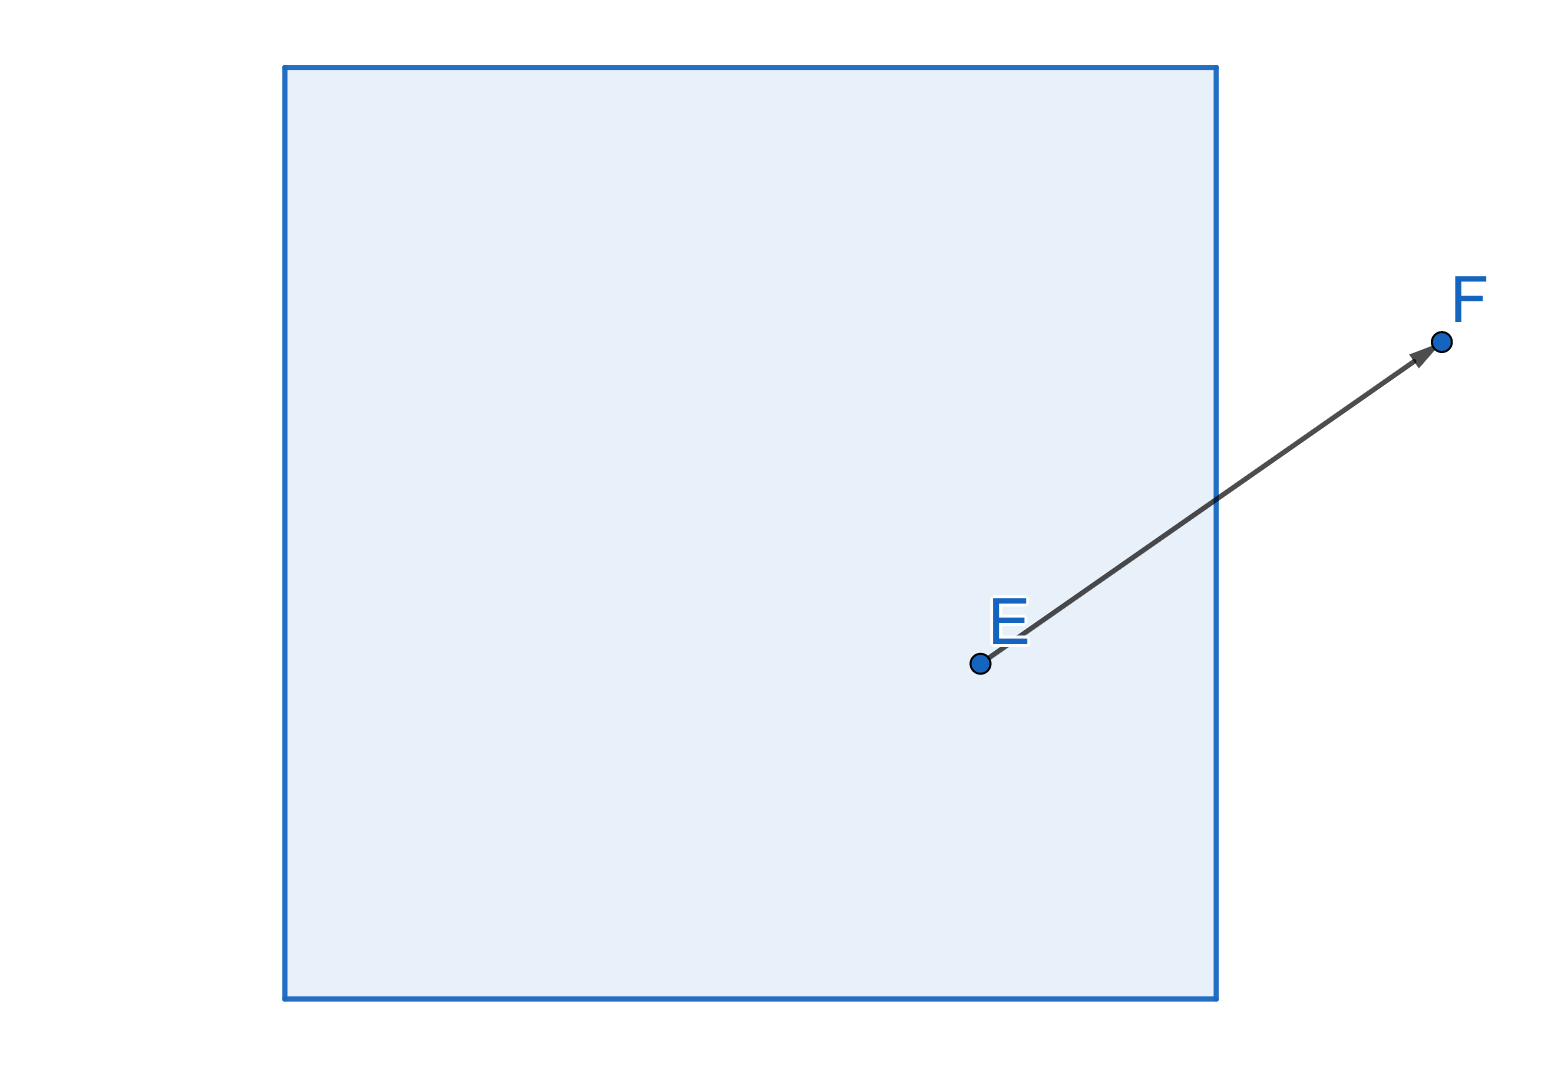
\includegraphics[width = 0.5\textwidth]{fig/intrusion_eg}
	\caption{An example of an \emph{intrusion}: at some random time, a node $E$ reproduces a new node spatially out side the origin block it belongs to. As shown in the figure, this quantity highly relies on the scale of this problem: if $r \ll \frac{L}{n}$, this probability will be approximately $0$. On the other hand, if $r$ is large enough, the probability will be meaningless since the odd that it landing on the same block will be zero. So this quantity is a good reflection of scaling property of the system. }\label{fig:intrusion_eg}
\end{figure}

The intrusion probability is defined as an arbitrary node produces a new node outside the block it belongs to. See the illustration in\@\ref{fig:intrusion_eg}.



The probability of intrusion can be implemented as follows, we temporarily set the geometric center of a square as the origin of a coordinate, and the $x$ and $y$ directions are set parellel to the edges of the block. We have 
\begin{align}
&P(\text{intrusion}) \\=& \int_{\vec{r}} p(\text{stepping out}|\vec{r})d\vec{r}\label{d1}\\
=& \int_{(x,y)} p(\text{stepping out}|\vec{r})dxdy    \notag \\
=& \int_{(x,y)}p(\text{x out or y out}|\vec{r})dxdy\notag
\\
=& \int_{(x,y)}p\left(r\cos\theta+x>\frac{L}{2}\text{ or }r\sin\theta+y>\frac{L}{2}|\vec{r}\right)dxdy,
\end{align}
where $\vec{r}=(x,y)$ represents the position that the old node is located, and $(r,\theta)$ is the relative position of the new node to the old node. The quantity $p\left(r\cos\theta+x>\frac{2}{L}|\vec{r}\right)$ equals to $p\left(\theta<\arccos\left(\frac{L/2-x}{r}\right)\right)$. From here, we can see that as the ratio $L/r$ is the determination of a species' intrusion. When  real life case is considered, $r$ varies across species. In this case, the ratio $L/r$ serves as the intrusion tendency of each species. 

The formula \@\ref{d1} derivated above tell us the \emph{arcsin} law of intrusion.

\subsection{Derivation for Zipf's law of urban rank sizes}

The wait time for the $n$th people in a city to be born since the $n-1$th is $\beta_2 \cdot \frac{1}{n-1}$. So inversely the expected population of a city at time $t$ is $e^{t/\beta_2}$. 

The more population a big city is, the more it is favored by up-comers. In study of city size distributions, SYM is a realization of \emph{the rich get richer} rule, for the city's growth rate increase proportionally with its present population. Thus, it is similar for cities size distributions to follow Zipf's law. 

We denote the sizes of cities at time $t$ as $n_i(t)$, for $i$ in $1,2,3,\dots$

We denote the expected population of a city initiated $t$ ago as $Z(t)$. The transition probability of $P(Z_t = j)$ is $e^{-\beta_2 t}(1-e^{-\beta_2 t})^{j-1}$. 

Using Kolmogorov’s Forward Equation
\begin{align}p_t'(1,j) = -\beta_2 j p_t(1,j) + \beta_2 (j-1) p_t(1,j-1).\label{forward}\end{align}  When $j = 1$, we have \[p_t'(1,1) = -\beta_2 p_t(1,1), \] which leads to $p_t=e^{-\beta_2}$. When $j>1$, we differentiate $P(Z_t = j)$ to have 
\begin{align}
	\frac{dP(Z_t = j)}{dt} &= -\beta_2e^{-\beta_2 t} (1-e^{-\beta_2 t})^{j-1} + e^{-\beta_2 t}(j-1)(1-e^{-\beta_2 t})^{j-2}\beta_2 e^{-\beta_2 t}\notag\\
	&= -\beta_2 e^{-\beta_2 t}(1-e^{-\beta_2 t})^{j-1} + e^{-\beta_2 t}(j-1)(1-e^{-\beta_2 t})^{j-2} [-(1-e^{-\beta_2 t})\beta_2+\beta_2]\notag\\
	&= -\beta_2 e^{-\beta_2 t}(1-e^{-\beta_2 t})^{j-1} -\beta_2 e^{-\beta_2 t}(j-1)(1-e^{-\beta_2 t})^{j-1} +\beta_2e^{-\beta_2 t}(j-1)(1-e^{-\beta_2 t})^{j-2}\notag\\
	&= -\beta_2 j e^{-\beta_2 t}(1-e^{-\beta_2 t})^{j-1} +\beta_2e^{-\beta_2 t}(j-1)(1-e^{-\beta_2 t})^{j-2}
\end{align}
which copes with equation \ref{forward}. Thus we complete the proof of the probability distribution of a city's population. The probability distribution of the region's population is easy to find according to the given result. The probability distribution of registering $j$ people in $i$ cities at time $t$, is \[ P_t(i,j) = \left(\begin{array}{c}{j-1} \\ {i-1}\end{array}\right)\left(e^{-\beta t}\right)^{i}\left(1-e^{-\beta t}\right)^{j-i}. \]

Moreover, tuning the mechanism from pure birth to birth-death process, we receive a different scaling facter.

\subsection{proof for Clark's law}

In this part, we use the mean-field approach to derive the spatial distribution of population within a species. This quantity can be interpreted as the spatial distribution mode of a species. 

The good thing about the mean-field approach is that we can use the potential concept to derive some conclusions. Here, we regard the growing mechanism as a multi-dimensional binary tree. On each dimension, the tree's $i$th layer has $i$ potential nodes. The probability on the $i$th node's generation is is the average of the two nearest nodes' potential generation probability, i.e. such a sequence,
\begin{align*}
(1)\\
(\frac{1}{2},\frac{1}{2})\\
(\frac{1}{4},\frac{1}{2},\frac{1}{4})\\
(\frac{1}{8},\frac{3}{8},\frac{3}{8},\frac{1}{8})\\
\dots
\end{align*}

finally we get the \emph{population decaying law} as 

Basing on the homogeneity of the choice of $\theta$, the derivation along different axis is the same. Within each city, the spatial distribution of people are captured by the mobility pattern of nodes, $(r,\theta)$. Clark's law\cite{clark1951urban} and some variations for multi-centered models\cite{griffith1981modelling} are empirical clues that correspond to such spatial distributions. Here we reformulate the Clark's law under spatial Yule principles. Since the isotropic setting, the derivation is only needed in one dimension added on a Doppler effect. When spatial constraints are neglected, the expected density distribution along an axis from the origin has an exponential form,$\rho (R)\sim e^{-\alpha R}$. We start the discussion as a node being placed on a broad area. Regardless of adding nodes on else axis, the second is placed at $r$ right-side of the first with a probability of $1/2$. Along this axis, the $n$th node is placed at $k$ from the right end with $C_n^k/2^n$. Using the Stirling formula, it approximately equals to \begin{align}
    & \frac{n^{n+1/2}}{\sqrt{2\pi}k^{k+1/2}(n-k)^{n-k+1/2}}\notag                         \\
=    & \frac{n-k}{k+1}\frac{(1+\frac{1}{n-1-k})^{-k-1/2}}{(1+\frac{1}{k})^{n-k-1/2}}\notag \\
=    & \frac{n-k}{k+1}\frac{(1+\frac{1}{n-1-k})^{n-k-1/2}}{(1+\frac{1}{k})^{k+1/2}}\notag  \\
\sim & e^{-k},
\end{align}
which turns out to be a exponential distribution. We can interpret it as the local properties of spatial Yule model is a discrete version of a maximum entropy system, since the Clark's law can also be derived by maximum entropy principle\cite{merity2009accurate}. Recalling the simple mobility assumption as random walk in random direction, we show that individual-level diffusion process can be approximated by the sum of really simple moves.This is a non-trivial result since this is not derived by mean field approach but by random walk assumption of human mobility. To make it precise, at the early stage of the process, a new community can land near the centre of an existing one. In reality, two communities that are too adjacent are sometimes illustrated as two \emph{districts} in the same city. In our model, a set of communities that destruct others' roundness functions the same with districts within one city. We run some numerical tests to examine our results. From the figure \ref{fig:clark}, we can see that neglecting the finite-sample effect, the main part of the distribution exhibits a well-behaving exponential decay along the axis from the origin of a community.

By alternating the distributions of step length, we can reproduce other forms of people density distributions. A more skewed distribution of $r$ brings a Levy-like mobility pattern. In particular, a power law mobility distribution brings a Zipf's density distribution $\rho '(R)\sim R^{-\gamma}$\cite{PhysRevX.4.011008}, where $\gamma$ is the scaling factor.  In the following part, we focus on global characteristics to derive the area and population distributions among communities.

On the other hand, we consider the individual level expansion at urban edges. We denote that the distance between the first and the furthest node of a city as $O$ and $F$, respectively, and the moment that $F$ lands its first offspring as $t+\tau$, where $t$ is the moment that $F$ is landed. We investigate the radius of the city, which is defined by the distance between $O$ and $F$. The radius of a city at time $t$, $R_t$, changes to $R_{t+\tau}$ when the offspring is given birth. The expectation of $R_{t+\tau}$ goes as 
\begin{align}
	E R_{t+\tau} &= \int_0^{\frac{\pi}{2}} \sqrt{(R_t+r\cos\theta)^2+(r\sin\theta)^2} d\theta \notag \\
	&= \sqrt{2 R_t r} \int_{0}^{\frac{\pi}{2}} \sqrt{\frac{R_{t}}{2 r}+\frac{r}{2 R_{t}}+\cos \theta} d \theta \notag\\
	&= 2(R_t+r) E\left(\pi/4| \frac{4R_t r}{(R_t+r)^2}\right)
\end{align}

\subsection{Numerical verification}

The decay ratio, to be specified, is inverse proportional to the step length of individual mobility, $r$. If we take the construction speed of a city as a constant, the city expands faster when the buildings are flat, which turns out to be the case that the variable $r$ is larger. In reality, Los Angeles is a perfect illustrator for this case while Manhattan tells the opposite tale of smaller $r$.

\begin{figure}[ht]
\centering
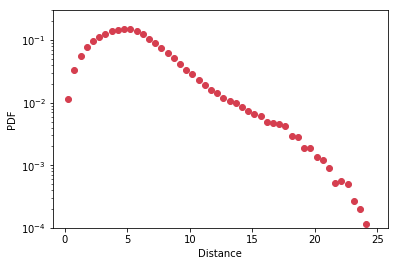
\includegraphics[width=0.9\linewidth]{fig/clark.png}
\caption{The population distribution as a function of distance from a district's center. The vertical axis is logarithmic processed, which represents the exponential decaying of population distribution. Regardless of the finite-sample effect, we fit the middle part of population density's spatial distribution to the exponential distribution with a slope of $-0.95$, which approximately equals to $1-1/\beta.$ This fit has a confidential measurement of $R^2=0.99$.}
\label{fig:clark}
\end{figure}

\subsection{Fractality}

The spatial competition is completed through the order of comers in edging areas. In this part, we derive two results related to the competition for space. First we consider the direct competition between the boundaries of two cities, which is determined by the population density at the edge of each city. Then we statistically test the fractal property of the \emph{urban envelope}. 

The spatial competition between cities can be abstracted as follows: the ownership of 

\section{Spatial coherence}

\section{Phase two: resource restrictions}

\subsection{superior switching} 

Regional development is complex and is affected by different determinants in different time. For example, in Hebei province of China, the largest city Shijiazhuang started to develop fast since it is the crossroad of railways. We interpret this as the redistribution of social resource. 

There have been plenty of literature\cite{bowles2019neolithic} that illustrate the interplay between social development and injustice. Social development 

Regional development is complex and is affected by differnet determinants in different time. For example, in Hebei province of China, the largest city Shijiazhuang started to develop fast since it is the crossroad of railways. Jilin City in Jilin province used to be the capital of Jilin province until Changchun, from 1954, replaced its status. Obviously, these are redistributions of social resource. In many literature, social injustice is strengthened by the techniacal revolutions. Stately, agricultural society is more likely to store fortune overtime than nomadic society\cite{doi:10.1086/701789}. The Gini coefficients in ancient society is also increasing as the productivity grows\cite{kohler2017greater}. We read this as inequality of human society is born with the desire of better life. 

But what is more interesting is that, when doesn't the rich get richer? In this Letter we give a possible explanation that the \emph{memory} of human society is the force of future endeavour. A city's future ability to develop is based on the active population brought by the existing active people. The limited resource is dynamically divided by increasing number of cities, so that there is, though small, but still some odd of overturn. In the following text, we first derive an approximated solution of this problem. We denote the coins share in the $k$th largest city as $n_k$, and investigate the probability that the second largest city becoming the largest, $P_{\text{overturn}}$. In $m$ successive additions of meta-population from the moment $t_l$, the chance for $n_2(t_l+m)\ge n_1(t_l+m)$ is equivalent to the case that the city $2$ is picked $n_1(t_l)-n_2(t_l)$ times more than city $1$. The probability of $n_1(t_l)-n_2(t_l)$ picks of city $2$ in a row is $\frac{n_1!}{n_2!}/N^{n_1-n_2}$. Adding another step brings an probability of $n_1/N$ for $n_1$ to increase to $n_1+1$. So the process ends at $n_1(t_l)-n_2(t_l)+1$ steps is the former probability times $(n_1+1)/N$ and plus a expected latent step length. These process results in a power law distribution shown in the following figure.



\subsection{Urban shrinkage}

The urban development is a sequel of the spatial distribution of existing resource. Thus the preferential attachment is not only performed among people, but also on urban land-use. The concentration of urban resource result in urban shrinkage, indicating that the popular definition of resource distribution, say Gross Democratic Product (GDP), may not be the best indicator of regional fortune, since it is not a perfect indication of a place's future 

Urban shrinking is widely discussed in recent years. It is always referred with demographic changes such as decreasing fertility, aging, and out-migration\cite{haase2008urban}. In the comprehension of urban input-output framework, the governmental investment cannot follow up with the spatial growth of population. So the further investment can only go to \emph{active} area where recent comers to the cities are mostly found. 

We conduct a block-wise analysis.

\subsection{Relative relationship between urban memory and urban size}

We give a numerical tests for this discussion. 

The \emph{extinction} discussed here refers to the extinction in the memory kernel, rather than the extinction of the whole species. Let $P_n(t)$ be the probability at time $t$ that a species has a popularity of $n$, and $\mathbb{P}(t)$ be the vector with component $P_n(t),k = 1,2,3,\dots,N^*$. Thus the extinction dynamics can be derived by a discrete Markov Chain. We denote $\Pi_{i,j}$ as the probability that a species has $i$ realizations within the memory kernel. Then we have \begin{align*}
&\Pi_{n,n} = (1-p)[(n/N^*)^2+(1-n/N^*)^2]+p(1-n/N^*),\\
&\Pi_{n,n+1}=(1-p)\frac{n}{N^*}(1-\frac{n}{N^*}),\\ 
&\Pi_{n,n-1}=(1-p)\frac{n}{N^*}(1-\frac{n}{N^*})+p\frac{n}{N^*}.
\end{align*}
This transition probability is suitable for every species. So we have a forward equation $$ \mathbb{P}(t+1) = \mathbb{P}(t)\Pi, $$which can be further derive as \begin{align*}
\frac{d\mathbb{P}}{dt} = \mathbb{P}(t)(\Pi-1)
\end{align*}
defined as the master equation. 


\section{Empirical evidence}

In this section, we give a visual check of urban growth pattern for real life dynamics. To work on this purpose, we want to see if the urban formation in real life conforms our settings. Since the space occupancy process is Markovian, we only need to pick a initial state to start the simulation. To this end, we 

As our model can be interpreted as the mechanism that groups of people are attached to some certain places, we find that this process is a perfect representative for metropolitan area's development. We use the night-light data in 20 years to illustrate the validity of our model. 

The night-time light dataset is often used to visualize how the city is expanding through space. We found it extremely suitable for validating spatial Yule model. 

We designed a experiment as follows. We sample the night-time light patterns from different thresholds of brightness at a time $t_0$ to represent different economical levels. We set the population within each blocks with the initial population distribution at some time stamp. Secondly, we simulate our model for different time scale to reformulate the metropolitan area development through time. 

% \begin{thebibliography}{99}
%     % \bibitem{David:1970} H.A. David, H.N. Nagaraja, {\it Order statistics}  (John Wiley \& Sons, Inc., 1970).
%     % \bibitem{Massey:1951} F.J. Massey, {\it Journal of the American statistical Association} {\bf 46}, 68-78 (1951).
% \end{thebibliography}
\bibliographystyle{plain}
\bibliography{refs.bib}
    
\end{document}